\subsection{Secondary Review}

Another aspect of our study will attempt to verify whether using anomaly detection to discover outliers in our dataset will produce a better overall predictor for an assessment. It is therefore appropriate to gain insight into how such detection is handled by the research community. Firstly the field of class imbalance will be introduced and from that other concepts will be reviewed.

\subsubsection{Introduction}

He and Garcia (2008~\cite{he2008learning}) refer to the idea of intrinsic-based and extrinsic-based class imbalances. Intrinsic being the occurrence of a class skew due to the data itself and extrinsic being a possible skew due to reasons beyond the data. Examples of intrinsic imbalance include picking out the hopefully small number of spam emails from the multitude of daily emails received so that the recipient is not inconvenienced but also does not miss any email. Another would be in predicting ``churn'' within an insurer`s member base, the vast majority of members would usually roll their policy over around its renewal time but a small percentage would switch. The insurer needs to target these potential churners before they make their decision but in targeting too many of the members they run the risk of alienating more than they can hope to retain. An example of extrinsic imbalance being a break in the recording of the data brought about through some type of interruption. Another being the data is collected at set times within which the minority class is most prevalent. Physical failures such as power supply or storage space may also create artificial skews in the data. A final example of extrinsic imbalance being manifested due to a change in the process of gathering of the actual data.
\par
Although this work makes no distinction between intrinsic and extrinsic imbalance, it is the authors belief that extrinsic imbalance issues will prove to be very relevant to this work's existing industry dataset. The data collection process has changed over a number of years and is reliant on a repeatable standard line of enquiry from a human practitioner. As time moves on, practitioners change and if the standards are not strictly adhered to then over time the data becomes skewed through no other reason than change in interpretation. That being said intrinsic imbalance is also present within the dataset through the simple fact that some candidate's attributes will be underrepresented within the total pool.

% \section{Traditional class imbalance}

%[TODO explain RF etc and cite some papers]

\subsubsection{Traditional Methods}\label{sec:TradMethods}
Possible solutions to the traditional class imbalance issue are typically split into data level and algorithm level solutions as described in the work of Ali et al. (2015~\cite{ali2015classification}). The data level encompassing both data sampling and feature selection methods whilst the algorithm level includes cost sensitive and hybrid or ensemble applications.
\par
Typical data sampling, cost sensitive techniques include Random Over-Sampling (ROS) and Random-Under Sampling (RUS). Whereas typical algorithm level methods include amongst others fuzzy rule-based classification (Chi et al., 1996~\cite{chi1996fuzzy}).
\par
Over sampling described in \secref{subsec:OverSampling} and under sampling in \secref{subsec:UnderSampling} can be thought of as two sides of the same coin in that over-sampling involves expanding the minority class through repetition and thus increasing the occurrence of the class whereas under-sampling involves removing samples from the majority class and hence reducing its dominance on the overall classification. Whereas entries of the minority class maybe added either randomly or through some computed method the entries from the majority class tend to be removed randomly. In fact the process of adjusting the majority/minority class has been the subject of a lot of work in its own right (Khoshgoftaar et al., 2007  \cite{khoshgoftaar2007learning}; Van Hulse et al., 2007 \cite{van2007experimental}).
\par
Finally it should be remembered that although til now the reader may have assumed that it is possible to improve classification results at either the data or algorithm level the hybrid scenario is one in which some combination of both of these may help. One example of this would be the introduction of the Random Forest (RF) classifier which although based on the earlier Random Decision Forest also has the inclusion of Bagging techniques (Gislason et al., 2006 \cite{gislason2006random}).

\subsubsection{Over sampling}\label{subsec:OverSampling}
Two prevalent over sampling techniques are Random Over Sampling (ROS) (Zhang \& Li, 2014~\cite{zhang2014rwo}) and Synthetic Minority Over-Sampling Technique (SMOTE)  (Chawla et al., 2002~\cite{chawla2002smote}; Chawla et al., 2003 \cite{chawla2003smoteboost}; Han Wang \& Mao \cite{han2005borderline}). One common complaint of over sampling techniques is their propensity to create an ``over-fitting'' (Fig~\ref{fig:Oversampling}) issue whereby the training data is too heavily mimicked leading to a poor model predictor. This over-fitting concern however can be mostly overcome through the use of SMOTE (Fern\'{a}ndez et al., 2017~\cite{fernandez2017insight}). Another complaint is an even larger training dataset than initially considered useful. In looking at the amount to which a minority class should be inflated it may appear reasonable that obtaining a 50/50 split would be ideal but Japkowicz and Stephen (2002~\cite{Japkowicz2002}), Fawcett and Provost (1997~\cite{fawcett1997adaptive}) along with Estabrooks and Japkowicz (2001~\cite{estabrooks2001mixture}) offer a counter argument and show that such a split would not produce the most favourable results.

\tikzset{every picture/.style={line width=0.75pt}} %set default line width to 0.75pt        
\begin{figure}[htbp]
\centering

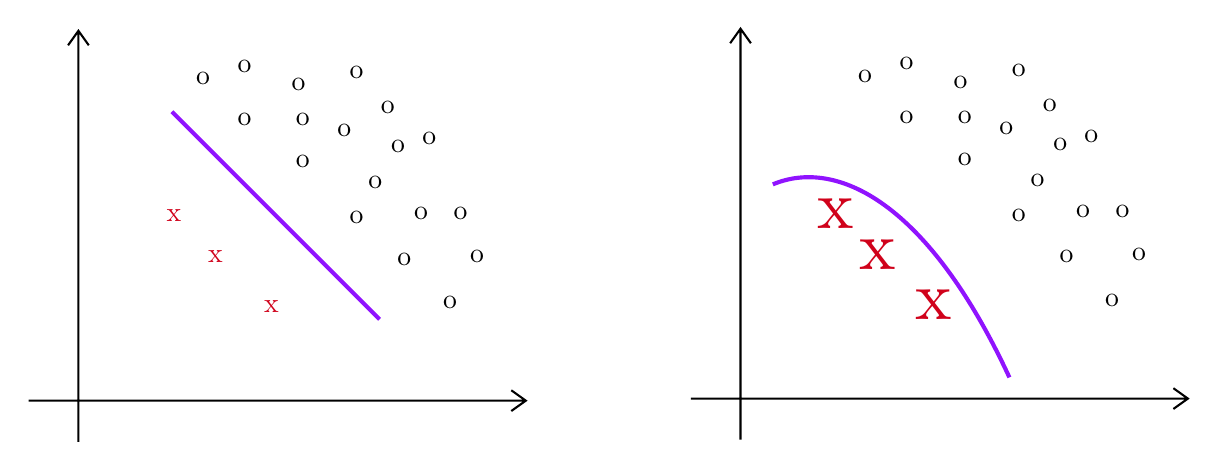
\begin{tikzpicture}[x=0.75pt,y=0.75pt,yscale=-1,xscale=1]
%uncomment if require: \path (0,300); %set diagram left start at 0, and has height of 300

%Shape: Axis 2D [id:dp33720031646484827] 
\draw  (50,215.2) -- (289.5,215.2)(73.95,37) -- (73.95,235) (282.5,210.2) -- (289.5,215.2) -- (282.5,220.2) (68.95,44) -- (73.95,37) -- (78.95,44)  ;
%Straight Lines [id:da49156386348114545] 
\draw [color={rgb, 255:red, 144; green, 19; blue, 254 }  ,draw opacity=1 ][fill={rgb, 255:red, 144; green, 19; blue, 254 }  ,fill opacity=1 ][line width=1.5]    (119,76) -- (219,176) ;


%Shape: Axis 2D [id:dp9978017465833935] 
\draw  (369,214.2) -- (608.5,214.2)(392.95,36) -- (392.95,234) (601.5,209.2) -- (608.5,214.2) -- (601.5,219.2) (387.95,43) -- (392.95,36) -- (397.95,43)  ;
%Curve Lines [id:da10887800526684499] 
\draw [color={rgb, 255:red, 144; green, 19; blue, 254 }  ,draw opacity=1 ][line width=1.5]    (408.5,111) .. controls (439.5,98) and (483.5,120) .. (522.5,204) ;



% Text Node
\draw (134,60) node  [align=left] {o};
% Text Node
\draw (154,80) node  [align=left] {o};
% Text Node
\draw (182,100) node  [align=left] {o};
% Text Node
\draw (180,63) node  [align=left] {o};
% Text Node
\draw (202,85) node  [align=left] {o};
% Text Node
\draw (217,110) node  [align=left] {o};
% Text Node
\draw (208,127) node  [align=left] {o};
% Text Node
\draw (231,147) node  [align=left] {o};
% Text Node
\draw (258,125) node  [align=left] {o};
% Text Node
\draw (253,168) node  [align=left] {o};
% Text Node
\draw (243,89) node  [align=left] {o};
% Text Node
\draw (208,57) node  [align=left] {o};
% Text Node
\draw (154,54) node  [align=left] {o};
% Text Node
\draw (182,80) node  [align=left] {o};
% Text Node
\draw (223,74) node  [align=left] {o};
% Text Node
\draw (239,125) node  [align=left] {o};
% Text Node
\draw (266,146) node  [align=left] {o};
% Text Node
\draw (228,93) node  [align=left] {o};
% Text Node
\draw (120,126) node [color={rgb, 255:red, 208; green, 2; blue, 27 }  ,opacity=1 ] [align=left] {x};
% Text Node
\draw (140,146) node [color={rgb, 255:red, 208; green, 2; blue, 27 }  ,opacity=1 ] [align=left] {x};
% Text Node
\draw (167,170) node [color={rgb, 255:red, 208; green, 2; blue, 27 }  ,opacity=1 ] [align=left] {x};
% Text Node
\draw (453,59) node  [align=left] {o};
% Text Node
\draw (473,79) node  [align=left] {o};
% Text Node
\draw (501,99) node  [align=left] {o};
% Text Node
\draw (499,62) node  [align=left] {o};
% Text Node
\draw (521,84) node  [align=left] {o};
% Text Node
\draw (536,109) node  [align=left] {o};
% Text Node
\draw (527,126) node  [align=left] {o};
% Text Node
\draw (550,146) node  [align=left] {o};
% Text Node
\draw (577,124) node  [align=left] {o};
% Text Node
\draw (572,167) node  [align=left] {o};
% Text Node
\draw (562,88) node  [align=left] {o};
% Text Node
\draw (527,56) node  [align=left] {o};
% Text Node
\draw (473,53) node  [align=left] {o};
% Text Node
\draw (501,79) node  [align=left] {o};
% Text Node
\draw (542,73) node  [align=left] {o};
% Text Node
\draw (558,124) node  [align=left] {o};
% Text Node
\draw (585,145) node  [align=left] {o};
% Text Node
\draw (547,92) node  [align=left] {o};
% Text Node
\draw (439,125) node [scale=2.488,color={rgb, 255:red, 208; green, 2; blue, 27 }  ,opacity=1 ] [align=left] {x};
% Text Node
\draw (459,145) node [scale=2.488,color={rgb, 255:red, 208; green, 2; blue, 27 }  ,opacity=1 ] [align=left] {x};
% Text Node
\draw (486,169) node [scale=2.488,color={rgb, 255:red, 208; green, 2; blue, 27 }  ,opacity=1 ] [align=left] {x};


\end{tikzpicture}

\caption{Oversampling} \label{fig:Oversampling}
\end{figure}


\subsubsection{Under sampling}\label{subsec:UnderSampling}
One of the most used under sampling (Fig~\ref{fig:Undersampling}) techniques is Random Under Sampling (RUS) (Seiffert et al., 2009~\cite{seiffert2009rusboost}). Good practice in the removal process from the majority class is that the data removed lies as far away from any boundary with the minority class as possible. Practitioners point out that one of the disadvantages of under sampling is the possible removal of valuable information from the core set and a possible change in the majority class's distribution if care is not taken in the extraction. For instance we could remove a large portion of young people from an otherwise well distributed cohort of data.




\tikzset{every picture/.style={line width=0.75pt}} %set default line width to 0.75pt       
\begin{figure}[htbp]
\centering


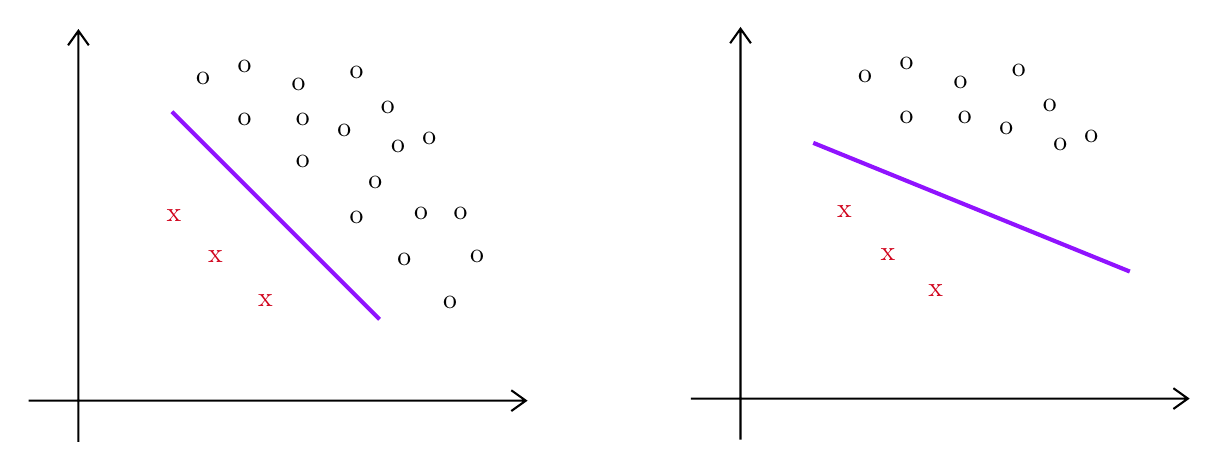
\begin{tikzpicture}[x=0.75pt,y=0.75pt,yscale=-1,xscale=1]
%uncomment if require: \path (0,300); %set diagram left start at 0, and has height of 300

%Shape: Axis 2D [id:dp33720031646484827] 
\draw  (50,215.2) -- (289.5,215.2)(73.95,37) -- (73.95,235) (282.5,210.2) -- (289.5,215.2) -- (282.5,220.2) (68.95,44) -- (73.95,37) -- (78.95,44)  ;
%Straight Lines [id:da49156386348114545] 
\draw [color={rgb, 255:red, 144; green, 19; blue, 254 }  ,draw opacity=1 ][fill={rgb, 255:red, 144; green, 19; blue, 254 }  ,fill opacity=1 ][line width=1.5]    (119,76) -- (219,176) ;


%Shape: Axis 2D [id:dp9978017465833935] 
\draw  (369,214.2) -- (608.5,214.2)(392.95,36) -- (392.95,234) (601.5,209.2) -- (608.5,214.2) -- (601.5,219.2) (387.95,43) -- (392.95,36) -- (397.95,43)  ;
%Straight Lines [id:da6705581541742359] 
\draw [color={rgb, 255:red, 144; green, 19; blue, 254 }  ,draw opacity=1 ][fill={rgb, 255:red, 144; green, 19; blue, 254 }  ,fill opacity=1 ][line width=1.5]    (428,91) -- (580.5,153) ;



% Text Node
\draw (134,60) node  [align=left] {o};
% Text Node
\draw (154,80) node  [align=left] {o};
% Text Node
\draw (182,100) node  [align=left] {o};
% Text Node
\draw (180,63) node  [align=left] {o};
% Text Node
\draw (202,85) node  [align=left] {o};
% Text Node
\draw (217,110) node  [align=left] {o};
% Text Node
\draw (208,127) node  [align=left] {o};
% Text Node
\draw (231,147) node  [align=left] {o};
% Text Node
\draw (258,125) node  [align=left] {o};
% Text Node
\draw (253,168) node  [align=left] {o};
% Text Node
\draw (243,89) node  [align=left] {o};
% Text Node
\draw (208,57) node  [align=left] {o};
% Text Node
\draw (154,54) node  [align=left] {o};
% Text Node
\draw (182,80) node  [align=left] {o};
% Text Node
\draw (223,74) node  [align=left] {o};
% Text Node
\draw (239,125) node  [align=left] {o};
% Text Node
\draw (266,146) node  [align=left] {o};
% Text Node
\draw (228,93) node  [align=left] {o};
% Text Node
\draw (120,126) node [color={rgb, 255:red, 208; green, 2; blue, 27 }  ,opacity=1 ] [align=left] {x};
% Text Node
\draw (140,146) node [color={rgb, 255:red, 208; green, 2; blue, 27 }  ,opacity=1 ] [align=left] {x};
% Text Node
\draw (164,167) node [color={rgb, 255:red, 208; green, 2; blue, 27 }  ,opacity=1 ] [align=left] {x};
% Text Node
\draw (453,59) node  [align=left] {o};
% Text Node
\draw (473,79) node  [align=left] {o};
% Text Node
\draw (499,62) node  [align=left] {o};
% Text Node
\draw (521,84) node  [align=left] {o};
% Text Node
\draw (562,88) node  [align=left] {o};
% Text Node
\draw (527,56) node  [align=left] {o};
% Text Node
\draw (473,53) node  [align=left] {o};
% Text Node
\draw (501,79) node  [align=left] {o};
% Text Node
\draw (542,73) node  [align=left] {o};
% Text Node
\draw (547,92) node  [align=left] {o};
% Text Node
\draw (443,124) node [color={rgb, 255:red, 208; green, 2; blue, 27 }  ,opacity=1 ] [align=left] {x};
% Text Node
\draw (464,145) node [color={rgb, 255:red, 208; green, 2; blue, 27 }  ,opacity=1 ] [align=left] {x};
% Text Node
\draw (487,162) node [color={rgb, 255:red, 208; green, 2; blue, 27 }  ,opacity=1 ] [align=left] {x};


\end{tikzpicture}

\caption{Undersampling} \label{fig:Undersampling}
\end{figure}

\subsubsection{Feature selection}
Feature selection is the process of selecting the most influential features for a given dataset to produce an improved classification process. While not solely related to imbalance conditions a consequence of better feature selection usually leads the betterment of the effects of such imbalances (Yin et al., 2013~\cite{yin2013feature}; Mladenic \& Grobelnik, 1999~\cite{mladenic1999feature}). A downside of using feature selection to reduce imbalance is the extra computational load that is required. The work undertaken by Mladenic and Grobelnik (1999~\cite{mladenic1999feature}) rates a number of feature selection ideas and puts the ``odds ratio'' ahead of the rest. This is confirmed in the work by Zhang et al (2018~\cite{zhang2018image}). This rating however is not confirmed in some works and the general belief is that feature selection is very much a case by case situation.

\subsubsection{Cost sensitive methods}
The general premise of cost sensitive methods is to assign a higher weight or prominence to a given occurrence of a minority classification than any majority one so as to boost the worth of the minority classifier and reduce the effects of any imbalance. Domingos (1999~\cite{domingos1999metacost}) and Elkan (2001~\cite{elkan2001foundations}) are early studies on this important topic. They rely upon something called a cost matrix (Table~\ref{tab:costmatrix}) which encapsulates all possible outcomes of a two class problem.

\begin{table}[htbp]
\centering
\begin{tabular}{|l|c|c|}
\hline
                 & \multicolumn{1}{l|}{actual negative} & \multicolumn{1}{l|}{actual positive} \\ \hline
predict negative & C(0, 0)                              & C(0, 1)                              \\ \hline
predict positive & C(1, 0)                              & C(1, 1)                              \\ \hline
\end{tabular}
\caption{Cost Matrix}
\label{tab:costmatrix}
\end{table}


An example given by Elkan (2001~\cite{elkan2001foundations}) of such a cost matrix would be in attempting to find a fraudulent credit card transaction (Table~\ref{tab:costmatrix_cc_example}). In this scenario approval of a fraudulent transaction would cost the provider the total amount or \textit{``-x''} whereas refusing the legitimate transaction would damage the provider's reputation with the client. Here Elkan suggests an arbitrary \$20 loss to be sufficient. Refusing a fraudulent transaction he attributes a \$20 benefit and finally a legitimate approval will cost the institution 2\% of the cost of the total amount or \textit{``x''}.

\begin{table}[htbp]
\centering
\begin{tabular}{|l|c|c|}
\hline
                 & \multicolumn{1}{l|}{fraudulent} & \multicolumn{1}{l|}{legitimate} \\ \hline
refuse & \$20                              & -\$20                              \\ \hline
approve & -x                              & -0.02x                              \\ \hline
\end{tabular}
\caption{Credit Card Fraud}
\label{tab:costmatrix_cc_example}
\end{table}


\subsubsection{Hybrid/ensemble methods}
Although these methods may also be considered a type of cost sensitive method the approach is quite different in that the result of the classification is some amalgam of multiple classifiers (Seiffert et al., 2009~\cite{seiffert2009rusboost}). Two very popular ensemble methods are Bagging and Boosting (Graczyk et al., 2010~\cite{graczyk2010comparison}). Bagging achieves its goals by producing more than a single training set with each set being uniquely classified. Each classification is then used to produce the final result. Boosting takes a similar divide and conquer approach as that of Bagging where multiple training sets are once again produced. The difference to Bagging is that the classification of each individual training set is weighted by the degree of error within that set so that the final combined result is induced by only the more favourable interim classifiers
\par


\par

\noindent
A first look at the collaborating company dataset suggests a very high class imbalance and so the work on limiting the effects through over or under sampling is particularly relevant to this research.

\subsubsection{Deep Learning Methods} \label{sec:Deep}
Now that the reader is aware of how it is possible to mitigate the affects of class imbalance using traditional methods we turn our attention to the use of deep learning within such imbalances. It should be reassuring to know that many of the sampling and cost methods already mentioned can be applied within a deep learning framework.
The work of Johnson and Khoshgoftaar (2019~\cite{johnson2019survey}) gives a thorough road map of influential papers in the field of deep learning with imbalanced classification.
Back in the 1990's Anand et al. (1993~\cite{anand1993improved}) researched ways in which the class imbalance issue could be resolved using shallow neural networks. The work describes how the majority class is responsible for swamping the net gradient of the dataset and hence has an overpowering affect on the final weights of the model.
\par
As in traditional methods we can split deep learning into data level, algorithm level and hybrid methods.
\par
\subsubsection{Data level}\label{subsec:DeepLearningDataLevel}
Hensman and Masko (2015~\cite{masko2015impact}) use a CNN to balance image data using ROS. The result of this is then in some ways contradicted by the work of Lee et al. (2016~\cite{lee2016plankton}) which suggests a CNN using RUS solves the imbalance issue more favourably. In the work of Pouyanfar et al. (2018~\cite{pouyanfar2018dynamic}) a completely new sampling method is introduced and once again a CNN using image data is proposed. The basic idea of this method is to over sample the minority while at the same time under sample the majority class. Further work by Buda et al. (2018~\cite{buda2018systematic}) compares RUS with ROS as well as two-phase learning again using image datasets. Their findings suggest that ROS is the most universal method for handling class imbalance whereas RUS is rated poor and two-phase learning with ROS and RUS being inferior to them being used individually. Two-phase learning has also been undertaken in the work of Lee et al. and shown to improve minority classification without affecting that of the majority class. It achieves this by only taking instances of the majority class during the pre-training phase so that the minority class is more influential at this phase but when the final training occurs the model is allowed to see all data.
\par
\subsubsection{Algorithm level}\label{subsec:DeepLearningAlgoLevel}
Custom loss functions are widely considered to be the easiest way to address class imbalance as unlike data level methods they do not increase the dataset size or training times, another advantage is that they do not require pre-processing steps. Much research has focused on their use within deep learning and many approaches exist. The work of Wang et al. (2016~\cite{wang2016training}) and Lin et al. (2017~\cite{lin2017focal}) created new loss functions, allowing minority classes to become larger contributors to the overall loss. Wang et al. created a custom loss function using deep MLPs. They firstly demonstrate why a mean square error (MSE) loss function is unsuitable because of the dominance of the majority class to affect the function. After this they propose two new loss functions being the mean false error (MFE) and mean squared false error (MSFE) which they then go on to show give a better balance between the majority and minority classes. In fact, most notably they outperform MSE more when the imbalance is more pronounced. Lin et al. (2017~\cite{lin2017focal}) on the other hand, introduce a focal loss (FL) in their custom implementation which is designed purely to help in classifying imbalances between the foreground and background objects in an image. Wang et al. (2018~\cite{wang2018predicting}), Khan et al. (2017~\cite{khan2017cost}) and Zhang et al. (2016~\cite{zhang2016training}) all studied cost sensitive DNNs in various guises with those proposed by Khan et al. with Zhang et al. having the extra bonus of obtaining cost matrices through training. Zhang et al. (2018~\cite{zhang2018image}) introduce a truly hybrid approach with transfer learning, CNN feature extraction and a nearest neighbour idea to improve imbalanced classification. Wang et al. (2018~\cite{wang2018predicting}) proposes something called a cost sensitive deep neural network wherein traditional one-hot encoding is superseded with ``categorical feature embedding''. The embedding along with extracted features through the use of a CNN are then used as input to a DNN for the final classification. Khan et al. (2017~\cite{khan2017cost}) introduce a custom method CoSen CNN, which learns both weighted parameters and misclassification costs during training. One major advantage of this is that the transfer learning approach within the CoSen method negates the requirement to choose an appropriate domain specific cost matrix. Consequently, no potentially expensive domain expert is required.
\par
\subsubsection{Hybrid methods}\label{subsec:DeepLearningHybridMethods}
A number of key works have presented their findings where they combine data and algorithm level methods. Each of these concentrate their efforts solely on the use of image datasets. Huang et al. (2016~\cite{huang2016learning}) introduce something called a ``Large Margin Local Embedding'' (LMLE) method which is claimed to generate fairer class sampling. This is achieved through the rationale that minority classes are typically sparse and can be populated easily with samples from another denser class. The downside of this approach is that it is both complicated and expensive to implement and as such would probably deter its future use. Ando and Huang (2017~\cite{ando2017deep}) propose the first Deep Over Sampling (DOS) method. The method maintains two parallel learning procedures wherein a lower layer is used to deduce an embedding function and the upper layer then uses this function to classify the imbalanced data. Dong et al. (2018~\cite{dong2018imbalanced}) uses a novel loss function combined with hard sample mining. The authors themselves suggest that this approach may only be appropriate within large datasets. It is a progressive classifier whereby members from the minority class that are deemed to have more affect on each mini batch are selected. This means each mini batch requires smaller amounts of data to train compared to using the whole dataset. As each mini batch is trained in turn the authors attempt to rectify the class imbalance incrementally giving the minority class more say in the final result.

\subsubsection{Related research topics and challenges} \label{sec:TopicsAndChallenges}
It is possible for classification imbalance to contain very high imbalance ratios. Indeed when the ratio does become excessively high it is sometimes more appropriate to think of the issue as not so much an imbalance one but as an anomaly detection issue. Within anomaly detection we assume that our dataset has an expected distribution and that anything that deviates sufficiently is an anomaly. The methods for such detection may differ from that of classification imbalance and so will not be discussed further in this review. They include clustering methods, one class SVM's and Isolation Forests. Our industry dataset has not to date been considered to contain an anomalous minority condition.
\par
% \section{Dataset size}
In a landscape where we harvest more and more data in the hope of either gaining hindsight now or sometime in the future from that data the idea of ``big data'' has arisen. This big data phenomena has caused issues for traditional machine learning. One such issue is that a number of accepted algorithms used in the field are either not capable of dealing with big data or run too slowly. They may have been designed to see all the data at the same time or cannot be sped up through parallelism because of the way they have been implemented.
\par
It is pertinent however to distinguish between big data and non big data so that we may confirm whether any methods to improve upon any classification imbalance are suitable in both cases. Katal et al. (2013~\cite{katal2013big}) explains that big data does not as its name suggests only refer to the size of the data but variety (multi-typed), volume (size), velocity (capture rate), variability (inconsistent load payloads), complexity (multi- sourced) and value (worth to organisation).
\par
For our collaborating company, as it expands its global reach the need for staying abreast of the best practices for dealing with ``big data'' will become paramount. The expectation to become a ``source of truth'' to other entities will also create a maze of connected services each having to deal with very diverse data sources.
